\chapter{Datenmodellierung} % (fold)
\label{sec:datamodelling}
Um für das empirische Experiment eine Datenbasis zu schaffen benötigt es ein Datenmodell. Hierbei soll ein möglichst realistisches und flexibles Modell genutzt werden, zudem sollte dieses Verzweigungen aufweisen um verschiedene Abfragekomplexitäten abbilden zu können. In diesem Szenario (vgl. Abb. 3) handelt es sich um ein Projektmanagement-Tool. Es exestieren drei Klassen, welche über drei Beziehungen miteinander verbunden sind. Die Klasse Person modeliert einen Menschen, mit den Attributen Vorname, Nachname und E-Mail. Sie steht mit der Klasse Project in einer n:n-Beziehung, wodurch mehrere Projekte zu einer Person zugeordnet werden können, aber auch mehrere Personen an einem Projekt arbeiten können. In der Klasse Projekt werden nur der Titel und das Datum an welchem das Projekt erstellt wurde gespeichert. Ein Projekt steht in einer 1:n-Beziehung zur Klasse Issue. Dadurch kann einem Issue nur ein Projekt zugeordnet werden, ein Projekt kann aber mehrere Issues beinhalten. Issue speichert Daten wie etwa den Titel, das Erstellngsdatum, den Status und den Grund des Status des Issues. Issue besitzt eine n:n-Beziehung zu Person, wodurch ein Issue von mehreren Personen bearbeitet werden kann und eine Person in mehreren Issues arbeiten kann.
\vspace{1cm}
\label{sec:datenmodell}
\begin{figure}[h!]
	\centering
	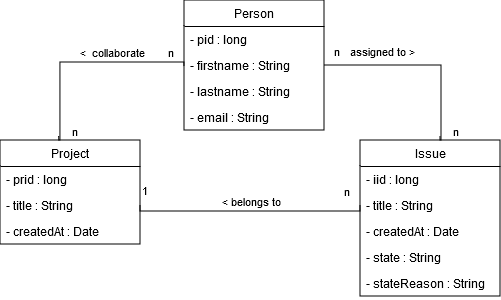
\includegraphics[scale=.8]{Illustrations/class_diagram.png}
	\caption{Klassendiagramm}
\end{figure}



% chapter datamodelling (end)

